\documentclass[a4paper,12pt]{report}

\usepackage{dependencias/ort}

% Este es el tamaño de margen que se usa en el documento.
\usepackage[left=3cm,right=3cm,top=3cm,bottom=3cm]{geometry}

% Filter out all marginpar warnings
%\usepackage{silence}
%\WarningFilter*{latex}{Marginpar on page \thepage\space moved}

\usepackage{pdflscape}
\usepackage[spanish, es-tabla, english]{babel}
\usepackage[below]{placeins}
\usepackage{fancyhdr}
\usepackage{enumerate}
\usepackage{blindtext}
\usepackage{multicol}
\usepackage{multirow}
\usepackage{etoolbox}
\usepackage{titlesec}
\usepackage[utf8]{inputenc}
\usepackage{csquotes}
\usepackage{graphicx}
\usepackage{array}
\usepackage[table,xcdraw]{xcolor}
\usepackage{booktabs}
\usepackage[pdftex,
    pdfauthor={Federico Alonso, Cristian Palma, Ramiro Gallego, Horacio Ábalos}, % DONE
    pdftitle={Sistema de Búsqueda y Rescate en el Mar}, % TODO
    pdfsubject={Tema}, % TODO
    pdfkeywords={Palabras clave}, % TODO
]{hyperref}
\usepackage{listings}
\usepackage{pdfpages}
\usepackage{enumitem}

% Subfigures and captions
\usepackage[figurename=Figura,tablename=Tabla]{caption}
\usepackage{subcaption}
\usepackage{xpatch}
\usepackage{hyperref}

\graphicspath{{images/}}
\titleformat{\chapter}{\normalfont\huge\bf}{\thechapter.}{20pt}{\huge}
\titlespacing*{\chapter}{0pt}{12pt}{12pt}


\makeatletter
\renewcommand{\l@section}{\@dottedtocline{1}{1.5em}{2.6em}}
\renewcommand{\l@subsection}{\@dottedtocline{2}{4.0em}{3.6em}}
\renewcommand{\l@subsubsection}{\@dottedtocline{3}{7.4em}{4.5em}}
\makeatother

\newcommand{\notAChapter}[1]{
%   \vspace*{2ex plus 1ex minus .2ex}
  \vspace*{12pt}  
  {\huge\bfseries #1}
  \vspace*{12pt}
}

\titleformat{\section}{\normalfont\LARGE\bf}{\thesection}{20pt}{\LARGE}
\titlespacing*{\section}{0pt}{12pt}{12pt}
\titleformat{\subsection}{\normalfont\Large\bf}{\thesubsection}{20pt}{\Large}
\titlespacing*{\subsection}{0pt}{12pt}{12pt}


% % % % % % % % % % % % % % % % % % % % % % % %  SUBSUBSECTION % % % % % % % % % % % % % % % % % % % % % % 
\titleformat{\subsubsection}
  {\normalfont\large\bfseries} % formato del título
  {\thesubsubsection} % número del título
  {1em} % espacio entre el número y el título
  {} % código anterior al título

% Opciones adicionales para el título
\titlespacing*{\subsubsection}{0pt}{12pt}{12pt}
% % % % % % % % % % % % % % % % % % % % % % % % % % % % % % % % % % % % % % % % % % % % % % 

% % % % % % % % % % % % % % % % % % % % % % % %  SUBSUBSUBSECTION % % % % % % % % % % % % % % % % % % % % % % 
% Definir el estilo de subsubsubsection sin afectar a paragraph
\newcommand{\subsubsubsection}[1]{%
  {\par\noindent\normalsize\textbf{#1}\par\normalsize}
}
% Ajustar el espaciado para el comando subsubsubsection similar a paragraph
\titlespacing*{\subsubsubsection}{0pt}{12pt}{12pt}

% % % % % % % % % % % % % % % % % % % % % % % % % % % % % % % % % % % % % % % % % % % % % % 

% Personalizar el estilo de paragraph y añadir un espacio después del título
\titleformat{\paragraph}[hang]
{\normalfont\normalsize\bfseries}
{\theparagraph}
{0em}
{}

\titlespacing*{\paragraph}{18pt}{12pt}{12pt}

\setcounter{tocdepth}{2} % Incluir hasta sub-subsecciones en el índice
\setcounter{secnumdepth}{3} % Numerar hasta sub-subsecciones

\renewcommand{\baselinestretch}{1.5}
\setlength{\parskip}{12pt}

\newcounter{paginas}
\setcounter{paginas}{1}
\usepackage{indentfirst}

\usepackage{color}
\definecolor{mygreen}{rgb}{0,0.6,0}
\definecolor{mygray}{rgb}{0.5,0.5,0.5}
\definecolor{mymauve}{rgb}{0.58,0,0.82}

\lstset{ %
    backgroundcolor=\color{white},
    basicstyle=\footnotesize,
    breakatwhitespace=false,
    breaklines=true,
    captionpos=b,
    literate={ó}{{\'o}}1 {ñ}{{\~n}}1,
    extendedchars=true,
    frame=single,
    keepspaces=true,
    keywordstyle=\color{blue},
    numbers=left,
    numbersep=5pt,
    numberstyle=\tiny\color{mygray},
    rulecolor=\color{mygray},
    showspaces=false,
    showstringspaces=true,
    showtabs=false,
    stepnumber=1,
    stringstyle=\color{mygreen},
    tabsize=2,
    title=\lstname
}

% Para definir colores:
% \definecolor{darkgray}{rgb}{.4,.4,.4}

\lstdefinelanguage{Javascript}{
    keywords={
        typeof, new, true, false, catch, function, return, null, catch, switch, var, if, in, while, do, else, case, break, export, private, async
    },
    keywordstyle=\color{blue}\bfseries,
    ndkeywords={class, export, boolean, throw, implements, import, this},
    ndkeywordstyle=\color{darkgray}\bfseries,
    identifierstyle=\color{black},
    sensitive=false,
    comment=[l]{//},
    morecomment=[s]{/*}{*/},
    commentstyle=\color{purple}\ttfamily,
    stringstyle=\color{red}\ttfamily,
    morestring=[b]',
    morestring=[b]"
}

\lstset{
    language=Javascript,
    extendedchars=true,
    basicstyle=\footnotesize\ttfamily,
    showstringspaces=false,
    showspaces=false,
    numbers=left,
    numberstyle=\footnotesize,
    numbersep=9pt,
    tabsize=2,
    breaklines=true,
    showtabs=false,
    captionpos=b
}

\usepackage[xindy,nonumberlist,nopostdot,style=altlist]{glossaries}
\makeglossaries

\newglossarystyle{mylist}{
    \setglossarystyle{listgroup}
    \renewenvironment{theglossary}
    {\begin{itemize}}{\end{itemize}}

    \renewcommand*{\glossentry}[2]{
        \item % bullet point
        \glstarget{##1}{\textbf{\glossentryname{##1}}:}% nombre
        \space \glossentrydesc{##1}% descripción
    }

    \renewcommand*{\glsgroupheading}[1]{
        \item[\textbf{\glsgetgrouptitle{##1}}]}
}

\usepackage[noabbrev,nameinlink,spanish]{cleveref}
\crefname{table}{tabla}{tablas}
\crefname{appendix}{Anexo}{Anexos}

\usepackage{pgfkeys}
\usepackage{longtable}

\usepackage[titletoc]{appendix}
% \titlecontents{<section>}[<left>]{<above>}
%               {<before with label>}{<before without label>}
%               {<filler and page>}[<after>]
    


\definecolor{mygreen}{rgb}{0,0.6,0}
\definecolor{mygray}{rgb}{0.5,0.5,0.5}
\definecolor{mymauve}{rgb}{0.58,0,0.82}

\lstset{ %
    backgroundcolor=\color{white},
    basicstyle=\footnotesize,
    breakatwhitespace=false,
    breaklines=true,
    captionpos=b,
    literate={ó}{{\'o}}1 {ñ}{{\~n}}1,
    extendedchars=true,
    frame=single,
    keepspaces=true,
    keywordstyle=\color{blue},
    numbers=left,
    numbersep=5pt,
    numberstyle=\tiny\color{mygray},
    rulecolor=\color{mygray},
    showspaces=false,
    showstringspaces=true,
    showtabs=false,
    stepnumber=1,
    stringstyle=\color{mygreen},
    tabsize=2,
    title=\lstname
}

\definecolor{darkgray}{rgb}{.4,.4,.4}
\definecolor{purple}{rgb}{0.65, 0.12, 0.82}
\definecolor{paleyellow}{RGB}{255, 253, 238}

\lstdefinelanguage{Javascript}{
    keywords={
        typeof, new, true, false, catch, function, return, null, catch, switch, var, if, in, while, do, else, case, break, export, private, async
    },
    keywordstyle=\color{blue}\bfseries,
    ndkeywords={class, export, boolean, throw, implements, import, this},
    ndkeywordstyle=\color{darkgray}\bfseries,
    identifierstyle=\color{black},
    sensitive=false,
    comment=[l]{//},
    morecomment=[s]{/*}{*/},
    commentstyle=\color{purple}\ttfamily,
    stringstyle=\color{red}\ttfamily,
    morestring=[b]',
    morestring=[b]"
}

\lstset{
    language=Javascript,
    extendedchars=true,
    basicstyle=\footnotesize\ttfamily,
    showstringspaces=false,
    showspaces=false,
    numbers=left,
    numberstyle=\footnotesize,
    numbersep=9pt,
    tabsize=2,
    breaklines=true,
    showtabs=false,
    captionpos=b
}

% define the key (arguments)
\pgfkeys{
    /sprint/.is family, /sprint,
    emptyParameter/.initial=,
    numero/.initial=,
    periodo/.initial=,
    objetivos/.initial=,
    planificacion/.initial=,
    cumplimiento/.initial=,
    resultados/.initial=
}

\usepackage{mathtools}
\setlength{\skip\footins}{10mm}


\newcommand{\checkmarkemoji}{
\includegraphics[height=1em]{imagenes/emojis/check.png}}
\newcommand{\crossemoji}{
\includegraphics[height=1em]{imagenes/emojis/cross.png}}

\usepackage[
    style=ieee,
    backend=biber,
    sorting=none
]{biblatex}

\DeclareFieldFormat{url}{[Online]. Available\addcolon\space\url{#1}}
\DefineBibliographyStrings{english}{
  urlseen = {Accessed on},
}

\DeclareFieldFormat{urldate}{%
  \bibstring{urlseen}%
  \addcolon\space%
  \ifcase\thefield{urlmonth}\or
  Jan.\or Feb.\or Mar.\or Apr.\or May\or Jun.\or
  Jul.\or Aug.\or Sep.\or Oct.\or Nov.\or Dec.\fi% Hardcodeado
  \addspace%
  \thefield{urlday}%
  \addcomma\addspace%
  \thefield{urlyear}%
}

\DefineBibliographyExtras{english}{
  \protected\def\mkbibmonth#1{%
    \ifcase#1\or
    Enero\or Febrero\or Marzo\or Abril\or Mayo\or Junio\or
    Julio\or Agosto\or Septiembre\or Octubre\or Noviembre\or Diciembre\fi}
}

\DeclareBibliographyDriver{online}{
  \usebibmacro{bibindex}%
  \usebibmacro{begentry}%
  \usebibmacro{author/editor+others/translator+others}%
  \setunit{\labelnamepunct}\newblock
  \printfield{title}%
  \printtext{,}% Inserta la coma inmediatamente después del título
  \iffieldundef{year}
    {}
    {\printtext{\addspace}%
     \printfield{month}\space\printfield{year}\addperiod}%
  \newunit\newblock
  \printfield{note}%
  \newunit\newblock
  \printlist{organization}%
  \newunit\newblock
  \printfield{version}%
  \newunit\newblock
  \usebibmacro{byauthor}%
  \newunit\newblock
  \usebibmacro{byeditor+others}%
  \newunit\newblock
  \printfield{howpublished}%
  \newunit\newblock
  \printfield{type}%
  \newunit\newblock
  \printfield{doi}%
  \newunit\newblock
  \printfield{url}%
  \newunit\newblock
  \printfield{urldateprefix}%
  \usebibmacro{urldate}%
  \usebibmacro{finentry}%
}





\addbibresource{./bibliografia/bibliois.bib}
\appto{\bibsetup}{\sloppy}
   
\pagestyle{fancy}
\renewcommand\headrulewidth{0pt}
\fancyhf{}
\fancyfoot[R]{\thepage}

\fancypagestyle{plain}{
    \renewcommand{\headrulewidth}{0pt}
    \fancyhf{}
    \fancyfoot[R]{\thepage}
}

% Estilo Caso de Uso
\newcommand\tabularhead[1]{
    \begin{table}[H]

        \begin{tabular}{|p{0.25\linewidth}|p{0.8\linewidth}|}
            \hline}

\newcommand\addrow[2]{#1 &#2\\ \hline}
\newcommand\addmulrow[2]{ \begin{minipage}[t][][t]{3cm}
                              #1
\end{minipage}%
    &\begin{minipage}[t][][t]{12cm}
         \begin{enumerate}
             #2
         \end{enumerate}
    \end{minipage}\\ \hline}

\newenvironment{casodeuso}{\tabularhead}
{\hline\end{tabular}\end{table}}

\newcommand{\completeref}[1]{\ref{#1}. \nameref{#1}}


\title{Sistema de Gestión de Búsqueda y Rescate en el Mar} 
\author{
    Federico Alonso - 182999\\
    Cristian Palma - 208443\\
    Ramiro Gallego - 135385\\
    Horacio Ábalos - 196991\\
}


% Se ordenan alfabéticamente de forma automática.

\newglossaryentry{Prueba}
{
    name=prueba,
    description={descripción}
}




\begin{document}
    \maketitle
    % textidote: ignore begin
    \addtocounter{page}{1}
    % textidote: ignore end

    \notAChapter{Declaración de autoría}\label{ch:declaracion-de-autoria}


    \notAChapter{Agradecimientos}\label{ch:agradecimientos}

    \notAChapter{Abstract}\label{ch:abstract}


    \notAChapter{Palabras clave}\label{ch:palabras-clave}

    % textidote: ignore begin
    \addtocontents{toc}{\protect\setcounter{tocdepth}{-10}}
    \clearpage
    \phantomsection
    \addcontentsline{toc}{chapter}{Glosario}
    \setglossarystyle{mylist}
    \printglossary[title={\-\hspace{18pt}Glosario}]
    \glsaddall
    \addtocontents{toc}{\protect\setcounter{tocdepth}{2}} % Restaurar el valor original de tocdepth
    % textidote: ignore end

    \renewcommand{\contentsname}{Índice}
    % textidote: ignore begin
    \tableofcontents
    % textidote: ignore end

    \chapter{Introducción}\label{ch:introduccion}

El propósito del presente documento es describir el proyecto de grado titulado “Sistema de Gestión de Incidentes de Búsqueda y Rescate en el Mar” para la Armada Nacional, realizado en el marco de los requerimientos para obtener el título de Ingeniero y Licenciado en Sistemas de la Universidad ORT Uruguay, bajo la tutoría del Ing. Juan Pablo Russo. El mismo fue llevado a cabo en el transcurso de marzo de 2024 a marzo de 2025 por los estudiantes descritos en la siguiente sección. 

% Cita a bibliografía \cite{JWT}

\section{Prueba}\label{sec:prueba}

\chapter{Descripción del Problema y la Solución}\label{ch:descripcionProblemaYSolucion}

% Cita a bibliografía \cite{JWT}

\section{Contexto}\label{sec:contexto}

Como se observa en la Figura\ref{fig:area_responsabilidad_armada}, el Uruguay, tiene asignada como región de responsabilidad, un segmento de la Zona 5 – Atlántico Sudoccidental, 
zona que comparte con la Rep. Argentina, la Rep. Federativa del Brasil y el Reino Unido. Esta área, que limita en su extremo Este \footnote{Longitud 010º W} con el área de responsabilidad de Sudáfrica, 
representa una superficie aproximada de 516.000 millas náuticas cuadradas\footnote{Esto equivale a \(1.770.000\ \text{km}^2\)}, equivalente a unas 10 veces el tamaño de la superficie terrestre de nuestro país.\\

\begin{figure}[!h]
    \centering
    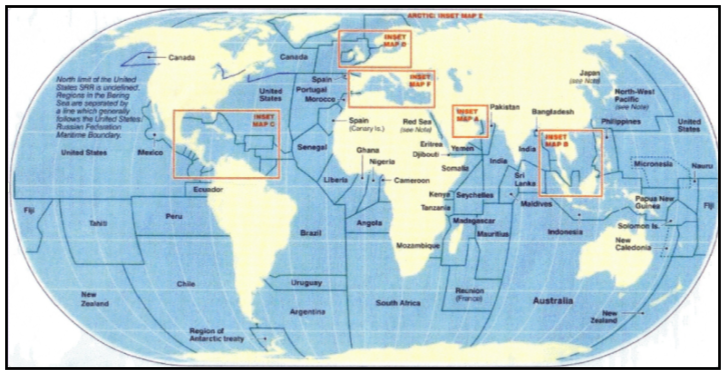
\includegraphics[width=\textwidth]{../imagenes/secciones/2-descripcion-del-problema-y-solucion/Regiones De Responsabilidad SAR.png} % Ancho total del texto
    \caption{Área de responsabilidad de la Armada Nacional}
    \label{fig:area_responsabilidad_armada}
\end{figure}


\FloatBarrier

\section{Descripción del Problema}\label{sec:descripcionDelProblema}

Actualmente el MRCC no cuenta con un sistema centralizado de gestión de incidentes, provocando que, cuando se produzca un siniestro, 
se generen ciertas ineficiencias como por ejemplo:

\begin{itemize}
    \item Demoras en las notificaciones a los involucrados;
    \item Demoras en procesamiento de los incidentes;
    \item Dificultad para la toma de decisiones.
    \item Excesiva concentración en el seguimiento del incidente, lo que les impide enfocarse en otras tareas.
    \item Acceso limitado o demorado de información técnica para los involucrados, por ejemplo, los encargados 
    del incidente deben contar con información sobre los procedimientos y la legislación para cada evento particular.
\end{itemize}

Para ilustrar el problema, vamos a examinar un escenario hipotético: un velero que viaja desde Colonia a Piriápolis se 
enfrenta a una tormenta repentina. Durante la tormenta, el miembro más capacitado de la tripulación para navegar sufre un 
accidente y queda inconsciente por lo cual requiere atención médica y a su vez deja al resto de la tripulación sin saber su 
ubicación precisa. El MRCC recibe esta información y se genera un incidente.\\
Antes de enviar un medio SAR al rescate, teniendo en cuenta la última posición conocida y el recorrido que tenía previsto realizar 
el barco del incidente, la guardia del MRCC busca información del tráfico marítimo en un sistema llamado \textit{SEA VISIÓN}, 
e intenta comunicarse con los mismos para ordenarles que asistan al velero.\\
En caso de no poder localizarlo, a partir de la última posición conocida, los datos del viento y de las corrientes se procede hacer un 
cálculo de la posición probable, a través del uso de planillas Excel implicando una demora de alrededor de 20 minutos de un oficial 
entrenado.\\
Luego de hacer el cálculo, dependiendo del escenario del incidente y de los medios disponibles SAR, se realiza un patrón de búsqueda. 
Para el mismo uno de los elementos a tener en cuenta son los incidentes en ubicaciones similares \footnote{los cuales se encuentran archivados 
físicamente en papel, por lo cual se apela a la memoria y experiencia del oficial de guardia}.\\
A continuación, se confecciona un correo electrónico con los datos del incidente y el resultado del patrón de búsqueda y se envía a los medios SAR 
designados. Estos medios SAR designados, a su vez, tiene personal responsable por contactar a toda su tripulación citándolos a presentarse a bordo 
\footnote{dicha citación se realiza tripulante a tripulante, comenzando por quienes se encuentren más alejados geográficamente}. 
Cabe observar que la tripulación de la embarcación son pocos en caso de un buque pequeño, pero cerca de 100 (cien) en caso de un buque de mayor 
porte.\\
Una vez ya desplegados los medios SAR para realizar el rescate, los mismos envían información de su posición a intervalos regulares y también
se solicita información de viento y corriente a efectos de ir actualizando el cálculo con mayor precisión, lo cual implica un retraso  
considerando el tiempo empleado en su elaboración. Posteriormente, esta información es transmitida por radio, aunque también
–a veces– puede ser necesario primero transmitirla a una estación costera para luego ser retransmitida al MRCC, lo cual produce demoras que 
pueden llegar a ser significativas.\\
Una vez localizado el velero, se brinda asistencia según la situación específica. Esta asistencia puede implicar dirigirse hacia el 
embarcadero más cercano a un hospital para darle atención médica a los heridos, remolcar la embarcación si es necesario, solicitar la 
intervención de un helicóptero para evacuar heridos de emergencia mientras el velero es remolcado con el resto de la tripulación, o en 
algunos casos, el médico de la unidad puede encargarse de la atención médica a bordo.\\
Las decisiones sobre cómo proceder se toman considerando varios parámetros como la distancia al embarcadero y al aeropuerto, o la gravedad 
de las heridas, entre otros muchos. Todas las decisiones mencionadas son realizadas y coordinadas desde el MRCC basadas en los 
procedimientos establecidos los cuales contemplan las buenas prácticas del \textit{Manual Internacional IAMSAR}, para lo cual todos los miembros de 
la guardia deben conocer especialmente el CMS (Coordinador de la Misión Sar) quien es responsable de las decisiones que toma durante el 
incidente SAR.\\
Finalmente, una vez completada la operación, se realiza un informe detallado de los eventos ocurridos el cual se archiva físicamente en un 
bibliorato para futuras referencias.\\
Anualmente el MRCC atiende unos 700 incidentes, de los cuales en promedio 50 terminan con el despliegue de un equipo de rescate, de estos 
incidentes se contabilizan alrededor de 10 fallecidos por año.\\
Cabe destacar que para la realización de los procesos de coordinación el MRCC solo cuenta con 6 personas, por lo que la eficiencia en los 
recursos en términos generales es fundamental para el éxito de las operaciones.

\section{Principales Interesados}\label{sec:pricipalesInteresados}

El equipo llevó a cabo el estudio de los principales interesados del proyecto. Se identificaron distintos grupos de interés, 
y se evaluaron sus necesidades y expectativas puntuales en relación con la solución propuesta.\\
Se consideró el nivel de influencia que cada uno de estos tenía en el proyecto, de forma de asegurar que sus preocupaciones fueran 
tomadas en cuenta para garantizar su colaboración en la implementación de la solución.\\
Para hacer un estudio detallado de los interesados y evaluar sus necesidades y expectativas se realizó una \textit{matriz de interés e influencia}~\cite{projectmanagement_stakeholder_analysis} 
para categorizarlos en base a los siguientes criterios:


\begin{itemize}
    \item \textbf{Alta influencia -  Alto interés:} Estos son los interesados clave que tienen un gran poder y un alto interés en el 
    éxito del proyecto. Deben ser gestionados de cerca, involucrándose activamente en la toma de decisiones y manteniéndolos informados 
    de manera regular. Su apoyo es crítico para el éxito del proyecto.
    \item \textbf{Alta influencia - Bajo interés:} Aunque no están muy interesados en los detalles diarios del proyecto, su influencia es 
    alta, por lo que es importante mantenerlos satisfechos. Se debe proporcionar información suficiente para asegurarse de que estén 
    contentos con la dirección del proyecto, pero no abrumarnos con demasiados detalles.
    \item \textbf{Baja influencia - Alto interés:} Estos interesados tienen un gran interés en el proyecto pero poca influencia en su éxito 
    o fracaso. Es importante mantenerlos bien informados y asegurarse de que se sientan valorados, aunque no es necesario involucrarlos en 
    las decisiones clave.
    \item \textbf{Baja influencia - Bajo interés:} Estos interesados no tienen mucho poder ni interés en el proyecto. Se debe monitorear su 
    situación para detectar cualquier cambio en su nivel de influencia o interés, pero generalmente no requieren mucha atención ni recursos.
\end{itemize}

El resultado de la clasificación fue el siguiente:


% \section{Descripción de la Solución}\label{sec:descriptionDeLaSolucion}


Solución tecnológica que gestione los incidentes de búsqueda y rescate en el mar. Esta solución se debe centrar en proporcionar una gestión 
centralizada, integral y eficiente de los incidentes que permita optimizar los recursos, el personal y el tiempo empleado. Para lograrlo debe 
ser imprescindible la capacidad de centralizar y automatizar procesos críticos de la gestión actual de los incidentes tales como: 

\begin{itemize}
    \item Realizar los cálculos de manera rápida y precisa. 
    El tiempo que se ahorra en la realización de los cálculos, considerar factores cambiantes de ciertas variables (como viento y corriente) 
    y no introducir el factor del error humano representa una optimización de los recursos, permite una mejor adaptación de las estrategias, 
    una coordinación eficiente de los involucrados y aumenta significativamente las probabilidades de éxito en los incidentes de rescate;
    \item Gestión de múltiples incidentes en tiempo real. Este es un aspecto fundamental considerando la alta demanda de incidentes que maneja el MRCC;
    \item Visualización detallada en el mapa del plan de rescate y monitoreo de las embarcaciones en tiempo real. 
    \item Acceso a la bitácora inmediata. Mejora la coordinación y reduce los tiempos de comunicación interna y respuesta en la cadena de mando;
    \item Permitir la extracción de estadísticas y reportes. Se presenta como una posibilidad para realizar ajustes continuos y mejoras en las estrategias 
    de búsqueda y rescate teniendo como base los aprendizajes de cada iteración;
    \item Presentar un diseño arquitectónico con bases en la disponibilidad. Asegura la disponibilidad y confiabilidad del sistema, aspecto crítico en operaciones 
    en las que el tiempo es vital.
\end{itemize}
\chapter{Marco Metodológico}\label{ch:marcoMetodologico}

\section{Características del Proyecto}\label{sec:caracteristicasDelProyecto}

Al tratarse de un proyecto académico la variable tiempo es fija en el contexto de la triple restricción (Alcance, Tiempo , Costo), 
por lo tanto trabajaremos con el enfoque \textit{date driven}. Para elegir el ciclo de vida del proyecto, nos basamos en las siguientes características 
que fueron identificadas:

\subsection{Características del Clientes} 
\textbf{Descripción del cliente.}\\
El Capitán Hugo de Barros, es el Jefe del Centro de Operaciones Tácticas del Comando de la Flota. 
Allí se encuentra el Centro Coordinador de Búsqueda y Rescate en el Mar (MRCC), el cual opera bajo la administración de la Armada Nacional, 
una de las tres fuerzas que componen las Fuerzas Armadas Uruguayas, dirigidas por el Ministerio de Defensa. 
La misión del MRCC comprende la planificación, control, coordinación y ejecución de la totalidad de las operaciones marítimas de Búsqueda y 
Rescate en el área de jurisdicción de la Armada Nacional, a fin de preservar la salvaguardia de la vida humana en el mar, y es su competencia 
la coordinación de los siniestros protagonizados por cualquier tipo de nave o aeronave, en las aguas jurisdiccionales y de interés nacional del 
Río Uruguay, Río de la Plata, Océano Atlántico y aguas interiores de jurisdicción de la Armada.
En esa unidad, la Armada Nacional mantiene una guardia permanente, administrada por el capitán Hugo de Barros. 

\textbf{Cliente disponible.}\\
El cliente tiene muy buena disposición para poder colaborar durante todo el proyecto. Nuestro contacto principal hace un 
servicio de guardia de 24 horas cada 9 días en el puesto de trabajo donde se está realizando el proyecto.

\textbf{Conocimiento del dominio.}\\
El cliente tiene muy buena disposición para poder colaborar durante todo el proyecto. Nuestro contacto principal hace un 
servicio de guardia de 24 horas cada 9 días en el puesto de trabajo donde se está realizando el proyecto.



\subsection{Características del Producto} 

Requerimientos obligatorios que pueden llegar a ser complejos por lo que a continuación se describe:

\textbf{Naturaleza Única de Cada Incidente.}\\
Cada incidente de búsqueda y rescate es único, con su propio conjunto de variables y desafíos, desde las condiciones 
climáticas y corrientes marinas hasta las características específicas de la embarcación en peligro y su tripulación. 
No hay dos incidentes que sean iguales y por lo tanto, la causa y efecto se pueden comprender claramente solo después de que 
se ha respondido al incidente.

\textbf{Ambigüedad y Dinamismo de las Condiciones Marítimas.}\\
Las condiciones marítimas son inherentemente impredecibles y cambiantes. La relación entre las acciones de búsqueda y rescate 
y sus resultados no siempre es predecible, y el éxito de una misión puede depender de factores inesperados que solo se revelan 
a través de la experiencia y el análisis retrospectivo.\\

\textbf{Conocimiento del dominio.}\\
El cliente tiene muy buena disposición para poder colaborar durante todo el proyecto. Nuestro contacto principal hace un 
servicio de guardia de 24 horas cada 9 días en el puesto de trabajo donde se está realizando el proyecto.
Existen una serie de requerimientos flexibles que pueden ser implementados de forma opcional, los cuales en gran medida fueron 
propuestos por el propio equipo dado que 3 de los miembros tienen experiencia de 15 años en la Armada Nacional lo cual 
facilitó tener una visión funcional y técnica al mismo tiempo.


\subsection{Características del equipo} 
\textbf{Tamaño del equipo.}\\
Somos un equipo de 4 miembros de las carreras Ingeniería en Sistemas y Licenciatura en Sistemas, lo cual fortalece las 
habilidades como  grupo. Al ser un equipo reducido es necesario contar con una buena organización y seleccionar herramientas 
de gestión y comunicación para facilitar la coordinación durante todo el proyecto.

\textbf{Experiencia del equipo en la Armada Nacional.}\\
Como se mencionó anteriormente, 3 miembros del equipo trabajaron en la Armada Nacional durante 15 años, lo cual hace que 
conozcamos bastante el dominio. También estos miembros del equipo formaron parte del Servicio de Informática de la Armada, 
lo cual implica que se conoce en detalle la arquitectura y tecnologías requeridas por el cliente.

\section{Metodología de Trabajo}\label{sec:metodologiaDeTrabajo}

\subsection{Ciclo de vida} 

Teniendo en cuenta las características del proyecto y las características del equipo se decidió utilizar un ciclo de vida 
incremental.  Dado que el conocimiento en el dominio y en las tecnologías utilizadas por el cliente nos permiten poder obtener 
al principio del proyecto la definición de los requerimientos y la arquitectura.

El proyecto se dividió en dos etapas:

\textbf{Discovery.}\\
Utilizando la metodología \textit{Design Thinking} y el marco de gestión Kanban con el objetivo de relevar los requerimientos a ser ejecutados 
en los primeros \textit{sprint} y también para definir la arquitectura durante un \textit{sprint} 0 en los meses de abril, mayo y junio. 

\textbf{Delivery.}\\
Para cada iteración de duración fija de dos semanas entre los meses de julio a diciembre realizaremos el diseño, codificación y pruebas de forma 
incremental adaptando el marco de gestión \textit{scrum}.

Se utilizará la metodología \textit{Dual Track Scrum} con algunas adaptaciones, porque entendemos que algunos requerimientos podrían requerir de actividades 
de \textit{discovery} durante el proyecto. Se evaluó utilizar solamente \textit{scrum} pero se decidió complementar el inicio generando un primer \textit{backlog} para 
alimentar sus iteraciones con una primera fase de \textit{discovery} a fin de mejorar la Ingeniería de Requerimientos.

    % textidote: ignore begin
    \addcontentsline{toc}{chapter}{Referencias bibliográficas}
    \printbibliography[title=Referencias bibliográficas]

    \nocite{*} % tiene que ir despues de printbiblio para q se ordene la bibliografia

    \chapter{Anexo}\label{ch:anexo}

% Definir un nuevo contador para los anexos
\newcounter{anexo}
\setcounter{anexo}{0} % Iniciar el contador en 0

% Configurar el formato de los títulos para incluir el prefijo de anexo
\newcommand{\anexoprefix}[1]{%
  \refstepcounter{anexo}% Incrementa el contador de anexos
  \thesection\ Anexo \arabic{anexo} - #1% Formato del título
}

% Antes de iniciar los anexos, cambia el formato de los títulos de sección
\titleformat{\section}
  {\normalfont\Large\bfseries}
  {}{0em}
  {\anexoprefix}


\section{Prueba}\label{anx:prueba-anexo}




   


    % textidote: ignore end

\end{document}
